\subsection{Синодический период}
\label{sec:synodic-period}

\term{Синодический период} (период смены фаз) небесного тела~--- период относительного кругового движения.

В большинстве случаев имеется в виду относительное движение планет вокруг Солнца (А). Также может рассматриваться период смены фаз спутника планеты (Б) или период между последовательными пролетами спутника над одним и тем же меридианом планеты (В).

Важным понятием в определении синодического периода является \imp{относительная угловая скорость}~--- скорость увеличения углового разделения двух рассматриваемых объектов. Так в случае (A) это скорость изменения угла <<{\slshape одна планета\,--\,Солнце\,--\,другая планета}>>, в случае (Б)~--- угла <<{\slshape спутник\,--\,планета\,--\,Солнца}>>, наконец, в случае (В)~--- угла между отрезком <<{\slshape центр планеты\,--\,спутника}>> и меридианом планеты.

Численно относительная скорость равна разности угловых скоростей двух рассматриваемых движений.
\begin{equation*}
    \boldsymbol\omega_\text{отн} = \boldsymbol{\omega}_1 - \boldsymbol\omega_2.
\end{equation*} 
Обозначим за $S$ синодический период, тогда
\begin{equation*}
    \frac{2\pi}{S} = |\boldsymbol\omega_\text{отн}| = |\vec\omega_1 - \vec\omega_2| = \left| \frac{2\pi}{T_1} \pm \frac{2\pi}{T_2} \right|,
\end{equation*}
где выбор знака в последнем выражении зависит от взаимного направления векторов угловых скоростей, а значит от направления каждого из движений. Окончательно, для синодического периода верно,
\begin{equation}
    \frac{1}{S} = \left| \frac{1}{T_1} \pm \frac{1}{T_2} \right|.
\end{equation}
   
Для внешних и внутренних планет, соответственно, выражения принимают вид:
\begin{equation} \frac{1}{S} = \frac{1}{T_\oplus} - \frac{1}{T_\text{пл}} \quad \text{и} \quad \frac{1}{S} = \frac{1}{T_\text{пл}} - \frac{1}{T_\oplus},
\end{equation}
где $S$~--- синодический период, $T_\text{пл}$~--- сидерический период планеты, $T_\oplus$~--- сидерический период обращения Земли.

\begin{figure}[h!]
    \centering
    \begin{subcaptionblock}[t]{0.32\tw}
        \centering
        \tikzsetnextfilename{synodic-period-same-direction-outer}
        \begin{tikzpicture}
            \tkzDefPoint(0,0){S}
            \def\R{1.1}
            \def\r{0.8}
            \def\OMEGAIN{40}
            \def\OMEGAOUT{\OMEGAIN * (\R/\r) ^ (-3/2)}
            \tkzDefShiftPoint[S](0,\r){IN}
            \tkzDefShiftPoint[S](0,\R){OUT}

            \tkzDrawCircle[black,line width=0.4pt](S,IN)
            \tkzDrawCircle[black,line width=0.4pt](S,OUT)

            \tkzDrawArc[rotate, semithick, -latex](S,IN)(\OMEGAIN)
            \tkzDrawArc[rotate, semithick, -latex](S,OUT)(\OMEGAOUT)

            \sun(S)
            \earth(IN)
            \tkzDrawPoint(OUT)
        \end{tikzpicture}
        \caption{Схема относительного движения Земли и объекта на внешней орбите, движущегося в том же направлении, что и Земля}
    \end{subcaptionblock}
    \hfill
    \begin{subcaptionblock}[t]{0.32\tw}
        \centering
        \tikzsetnextfilename{synodic-period-same-direction-inner}
        \begin{tikzpicture}
            \tkzDefPoint(0,0){S}
            \def\R{1.1}
            \def\r{0.8}
            \def\OMEGAIN{40}
            \def\OMEGAOUT{\OMEGAIN * (\R/\r) ^ (-3/2)}
            \tkzDefShiftPoint[S](0,\r){IN}
            \tkzDefShiftPoint[S](0,\R){OUT}

            \tkzDrawCircle[black,line width=0.4pt](S,IN)
            \tkzDrawCircle[black,line width=0.4pt](S,OUT)

            \tkzDrawArc[rotate, semithick, -latex](S,IN)(\OMEGAIN)
            \tkzDrawArc[rotate, semithick, -latex](S,OUT)(\OMEGAOUT)

            \sun(S)
            \tkzDrawPoint(IN)
            \earth(OUT)
        \end{tikzpicture}
        \caption{Схема относительного движения Земли и объекта на внутренней орбите, движущегося в том же направлении, что и Земля}
    \end{subcaptionblock}
    \hfill
    \begin{subcaptionblock}[t]{0.32\tw}
        \centering
        \tikzsetnextfilename{synodic-period-opposite-direction}
        \begin{tikzpicture}
            \tkzDefPoint(0,0){S}
            \def\R{1.1}
            \def\r{0.8}
            \def\OMEGAIN{40}
            \def\OMEGAOUT{\OMEGAIN * (\R/\r) ^ (-3/2)}
            \tkzDefShiftPoint[S](0,\r){IN}
            \tkzDefShiftPoint[S](0,\R){OUT}

            \tkzDrawCircle[black,line width=0.4pt](S,IN)
            \tkzDrawCircle[black,line width=0.4pt](S,OUT)

            \tkzDrawArc[rotate, semithick, -latex](S,IN)(\OMEGAIN)
            \tkzDrawArc[rotate, semithick, latex-](S,OUT)(-\OMEGAOUT)

            \sun(S)
            \earth(IN)
            \tkzDrawPoint(OUT)
        \end{tikzpicture}
        \caption{Схема относительного движения Земли и объекта, движущегося в противоположном направлении, нежели Земля}
    \end{subcaptionblock}
    \caption{}
\end{figure}

В случае, если тела обращаются в противоположные стороны, связь
их синодического периода с сидерическими очевидным образом принимает вид:
\begin{equation}
    \frac{1}{S} = \frac{1}{T_1} + \frac{1}{T_2}.
\end{equation}

\begin{wrapfigure}[14]{r}{0.47\tw}
    \centering
    \vspace{-1pc}
    \tikzsetnextfilename{sinodic-period-plot}
    \begin{tikzpicture}
        \begin{axis}[
            width    =    6cm,
            height    =    6cm,
            xlabel    =    {$T_2 / T_1$},
            ylabel    =    {$S / T_1$},
            ymax    =    6,
            ymin    =    0,
            xmax    =    6,
            xmin    =    0,
            legend cell align=left,
            legend style={
                row sep = 0.8pc,
                draw=none,
                fill=none,
                font=\scriptsize,
                at={(axis cs:2.5, 5.5)}, anchor=north west,
            },
        ]
            \addplot [domain=0:1, samples=100, black] {-1 / (1 - 1 / x)};
            \addplot [domain=1:6, samples=100, dash pattern=on 6pt off 2pt on 1pt off 2pt] {1 / (1 - 1 / x)};
            \addplot [domain=0:6, samples=100, dash pattern=on 6pt off 2pt on 1pt off 2pt on 1pt off 2pt] {1 / (1 + 1 / x)};

            \addplot [dashed, line width=0.5pt] coordinates { (1,0) (1,6) };
            \addplot [dashed, line width=0.5pt] coordinates { (0,1) (6,1) };

            \legend{
                $\dfrac{1}{T_1/T_2 - 1}$,
                $\dfrac{1}{1 - T_1/T_2}$,
                $\dfrac{1}{1 + T_1/T_2}$
            }
        \end{axis}
    \end{tikzpicture}
    \caption{}
    \label{pic:sinodic-period-plot}
\end{wrapfigure} 
На~\picRef{pic:sinodic-period-plot} изображены зависимости продолжительности синодического периода от отношения периодов планет. Важно обратить внимание на вертикальную асимптоту, к которой стремится график в случае движения планет в одну сторону вокруг Солнца. Она отражает отсутствие смены фаз в случае движения объектов по одной круговой орбите.

Горизонтальная асимптота является следствием стремления синодического периода к сидерическому периоду наблюдателя при стремлении сидерического периода объекта к бесконечности. При этом в случае сонаправленного движения синодический период приближается к сидерическому периоду наблюдателя сверху, а в случае встречного~--- снизу.

{\footnotesize Рассмотрим подробнее описанные выше случаи на конкретных примерах.\newline
{\bfseries (A) Относительное движение двух планет вокруг Солнца.} Для анализа возьмем пару Земля и Венера. Период Земли $T_\oplus = 1$~год, Венеры~--- $T_{\venus} = 0.62$~года. Следовательно, синодический период (период смены фаз) Венера для земного наблюдателя, также синодический период Земли для наблюдателя на Венера, определяется как
\begin{equation*}
    \frac{1}{S_{\oplus\venus}} = \left| \frac{1}{T_\oplus} - \frac{1}{T_{\venus}} \right| = \frac{1}{T_{\venus}} - \frac{1}{T_\oplus} = \frac{1}{0.62~\text{года}} - \frac{1}{1~\text{год}} = 0.61~\frac{1}{\text{год}}~~\Rightarrow~~S_{\oplus\venus} = 1.63~\text{года},
\end{equation*}
важно отметить, что здесь имеется в виду не календарный, а сидерический год Земли.\newline
{\bfseries (Б) Период смены фаз спутника планеты.} Найдём период смены фаз естественного спутника Земли~--- Луны. Движения, рассматриваемые в данном примере, это обращение Луны вокруг Земли с сидерическим периодом Луны $T_{\rightmoon} = 27.3$~суток и обращение Земли вокруг Солнца с сидерическим периодом Земли $T_\oplus \simeq 365$~суток. Следовательно, период смены фаз Луны
\begin{equation*}
    S_{\rightmoon} = \left| \frac{1}{T_\oplus} - \frac{1}{T_{\rightmoon}}\right|^{-1} = \left(\frac{1}{T_{\rightmoon}} - \frac{1}{T_\oplus}\right)^{-1} = \left(\frac{1}{27.3} - \frac{1}{365}\right)^{-1} = 29.5~\text{суток}.
\end{equation*}
{\bfseries (В) Орбитальное движение и вращение вокруг своей оси.} Несколько переиначим пример описанный выше: рассмотрим движение Земли вокруг Солнца и суточное вращение Земли вокруг своей оси, найдём продолжительность солнечных суток на Земле. Сидерический период Земли $T_\text{орб} \simeq 365$~суток (солнечных), а звёздные сутки $T_\text{ос} = 23^\text{h}\,56^\text{m}\,4^\text{s}$. Отсюда,
\begin{equation*}
    T_\text{сут} = \left(\frac{1}{T_\text{ос}} - \frac{1}{T_\text{орб}}\right)^{-1} = 24~\text{часа}.
\end{equation*}}

\subsubsection*{Либрация}

\begin{wrapfigure}[15]{r}{0.52\tw}
    \centering
    \vspace{-1pc}
    \tikzsetnextfilename{libration-plot}
     \begin{tikzpicture}
        \begin{axis}[
            width     =    6cm,
            height    =    6cm,
            ymax    =    3.142,
            xmax    =    6.284,
            xmin    =    0,
            ymin    =   -3.142,
            xlabel    =    {$M$},
            ylabel     =     {$\nu - M$},
            legend cell align=left,
            legend style={
                draw=none,
                fill=white,
                font=\scriptsize,
                at={(axis cs:3.5, 3)}, anchor=north west,
            },
            legend image post style={
                minimum height=0.75em,
                minimum width=3.5em,
            },
            xtick={0, pi / 2, pi, 3 * pi / 2, 2 * pi}, 
            xticklabels={$0$, $\pi / 2$, $\pi$, $3\pi / 2$, $2\pi$},
            ytick={-pi, -pi / 2, 0, pi / 2, pi}, 
            yticklabels={$-\pi$, $-\dfrac{\pi}{2}$, $0$, $\dfrac{\pi}{2}$, $\pi$},
        ]
            \addplot[smooth,dash pattern=on 6pt off 2pt on 1pt off 2pt on 1pt off 2pt on 1pt off 2pt] table[x=m, y=e01, col sep = comma] {data/libration.csv};
            \addplot[smooth,dash pattern=on 6pt off 2pt on 1pt off 2pt on 1pt off 2pt] table[x=m, y=e03, col sep = comma] {data/libration.csv};
            \addplot[smooth,dash pattern=on 6pt off 2pt on 1pt off 2pt] table[x=m, y=e05, col sep = comma] {data/libration.csv};
            \addplot[smooth,dash pattern=on 6pt off 2pt] table[x=m, y=e07, col sep = comma] {data/libration.csv};
            \addplot[smooth] table[x=m, y=e09, col sep = comma] {data/libration.csv};

            \legend{
                $e=0.1$,
                $e=0.3$,
                $e=0.5$,
                $e=0.7$,
                $e=0.9$,
            }
        \end{axis}
    \end{tikzpicture}
    \caption{}
    \label{pic:libration-plot}
\end{wrapfigure}
Tермин \term{либрация} в астрономии используется для описания влияния неравномерности орбитального движения спутника его на видимое вращение, которое происходит в постоянной угловой скоростью. В случае сихрнонизации орбитального движения спутника и его вращения вокруг оси, например, Луна, либрация позволяет наблюдателю на Земле видеть более половины поверхности спутника. 

Так как вращение спутника вокруг своей оси происходит с постоянной угловой скоростью, то оно линейным образом зависит от средней аномалии $M$ спутника. При этом средняя аномалия связана с эксцентрической аномалией $E$ уравнением Кеплера \eqref{eq:kepler-eq-E-nu-2}. Которая в свою очередь описывать истинную аномалию $\nu$, определяющую положение тела на орбите и, соотвветственно, его поворот относительно наблюдателя в следствии орбитального движения.

Выразим эксцентрическую аномалию $E$ как функцию от средней аномалии $M$. Для этого воспользуемся методом неподвижной точки\,\cite{balk_dynamic_space_flight}. Пусть $E_0 = 0$, а $E_{n+1} = e \sin E_n + M$, такая последовательность сходится, см.~\cite{balk_dynamic_space_flight}. Не сложно  получить, что
\begin{equation*}
    E_n = M + e \sin \big( M + e \sin ( M + \ldots) \big).
\end{equation*}
Далее преобразуем \eqref{eq:kepler-eq-E-nu-2}, чтобы получить выражение для $nu$:
\begin{equation*}
    \nu = 2 \arctg \left( \tg \frac{E}{2} \sqrt{\frac{1 + e}{1 - e}} \right).
\end{equation*}

Разность $\nu - M$ определяет разность между наблюдаемой ориентацией спутника и ориентацией в случае круговой орбиты. График зависимости $\nu - M$ от $M$ или, что тоже самое, от части периода спутника приведем на \picRef{pic:libration-plot} для различных величин эксцентриситета $e$.


